\chapter{软件的寻找与安装}
\label{software-installation}

\begin{intro}
  软件的下载安装一直以来是困扰许多「电脑小白」的大问题——从哪里下?怎么下?下完怎么装?装完怎么办?什么,软件要收费?破解是什么?……这一章将对国内互联网环境下 Windows 软件的下载、安装和配置做一个简单的介绍。看完这一部分,你或许可以找到下面这些问题的答案,并慢慢对「怎么寻找软件」有一个初步的了解。
  \begin{itemize}
    \item 我想下载 xxx 软件,我应该去哪里找这软件?
    \item 网上全是病毒和垃圾软件,我应该怎么样最大程度保证自己电脑的安全?
    \item 为什么软件下到手还要安装?有的还要破解?为什么这么麻烦?
    \item 电脑里不是有个「Microsoft Store」吗?为什么那里面大多数软件都找不到?
  \end{itemize}
\end{intro}

直到今天,Windows 系统下依然没有一个广泛使用的集中化「应用商店」。与我们使用手机不同,在电脑上,我们若想安装某个软件,多数情况下需要到互联网上寻找软件的「安装包」,再自行将软件「安装」到电脑上来使用。

这部分,我们将具体介绍软件为什么要「安装」,如何从网上的万千垃圾软件中下载我们需要的软件,以及软件安装和配置的一些技巧和注意事项。

\section{安装与安装包}

在 Windows 系统上,应用是通过「安装包」来安装到系统上的。如果把 app 比作是一株植物,那安装包就是这棵植物生长之前的「种子」。我们要安装某个 app,就需要获取这个 app 的安装包,然后通过安装包将 app「安装」在电脑上。

为什么需要「安装包」而不直接分发应用本身呢?我们有必要稍微了解一下 app 在我们的电脑上「安装」的过程。

在\nameref{files-and-file-management}中我们看到,一款 app 除了主程序(一个 \verb|exe| 文件)外,还包含一大堆不可或缺的依赖文件和子文件夹,如图 \ref{ncm-files} 所示。

\begin{figure}[htb!]
  \centering
  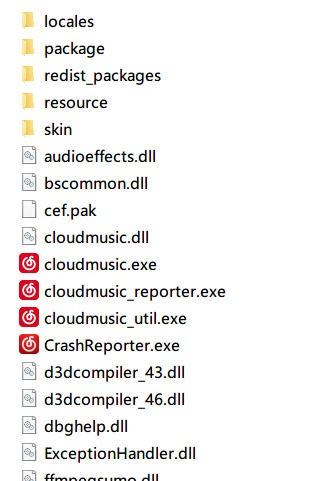
\includegraphics[width=5cm]{assets/Netease_cloud_music_files.png}
  \caption{「网易云音乐」的目录结构}
  \label{ncm-files}
\end{figure}

安装包的作用之一,便是把上面这一大堆文件按照它们能够工作的结构「释放」到我们的电脑中的指定位置。而除了「释放 app 的文件」之外,安装包还会做一些其他事情,例如设置一些文件的打开方式(上一章中提到的那张「表」)、调整一些系统内部的参数等。可以说,软件安装的过程,不仅仅是将一大堆文件「释放」或者说「提取」到系统中的某一个位置的过程,它还会对系统进行或多或少的调教与更改。这就是「安装包」存在的意义——它帮助我们完成了这复杂的「安装」过程。

\section{如何上网寻找软件的安装包}

下面我们来探讨如何上网寻找我们需要的软件的安装包。

\subsection{优先考虑:官方网站}

当要获取一款 app 时,我们首先应该考虑的是 app 开发者的官方网站,即「官网」。比起在其他地方下载软件,从官网下载软件能最大限度地保证你所下载的东西是干净的。

然而,\regcolor{对于百度这样的搜索引擎,官网常常不是搜索结果中的第一个——百度搜索出来的前 3 条结果一般是广告}。例如,我们想要下载「WPS」,直接在百度中搜索「WPS 下载」,我们会得到图 \ref{baidu-wps-result} 那样的搜索结果。

\begin{figure}[htb!]
  \centering
  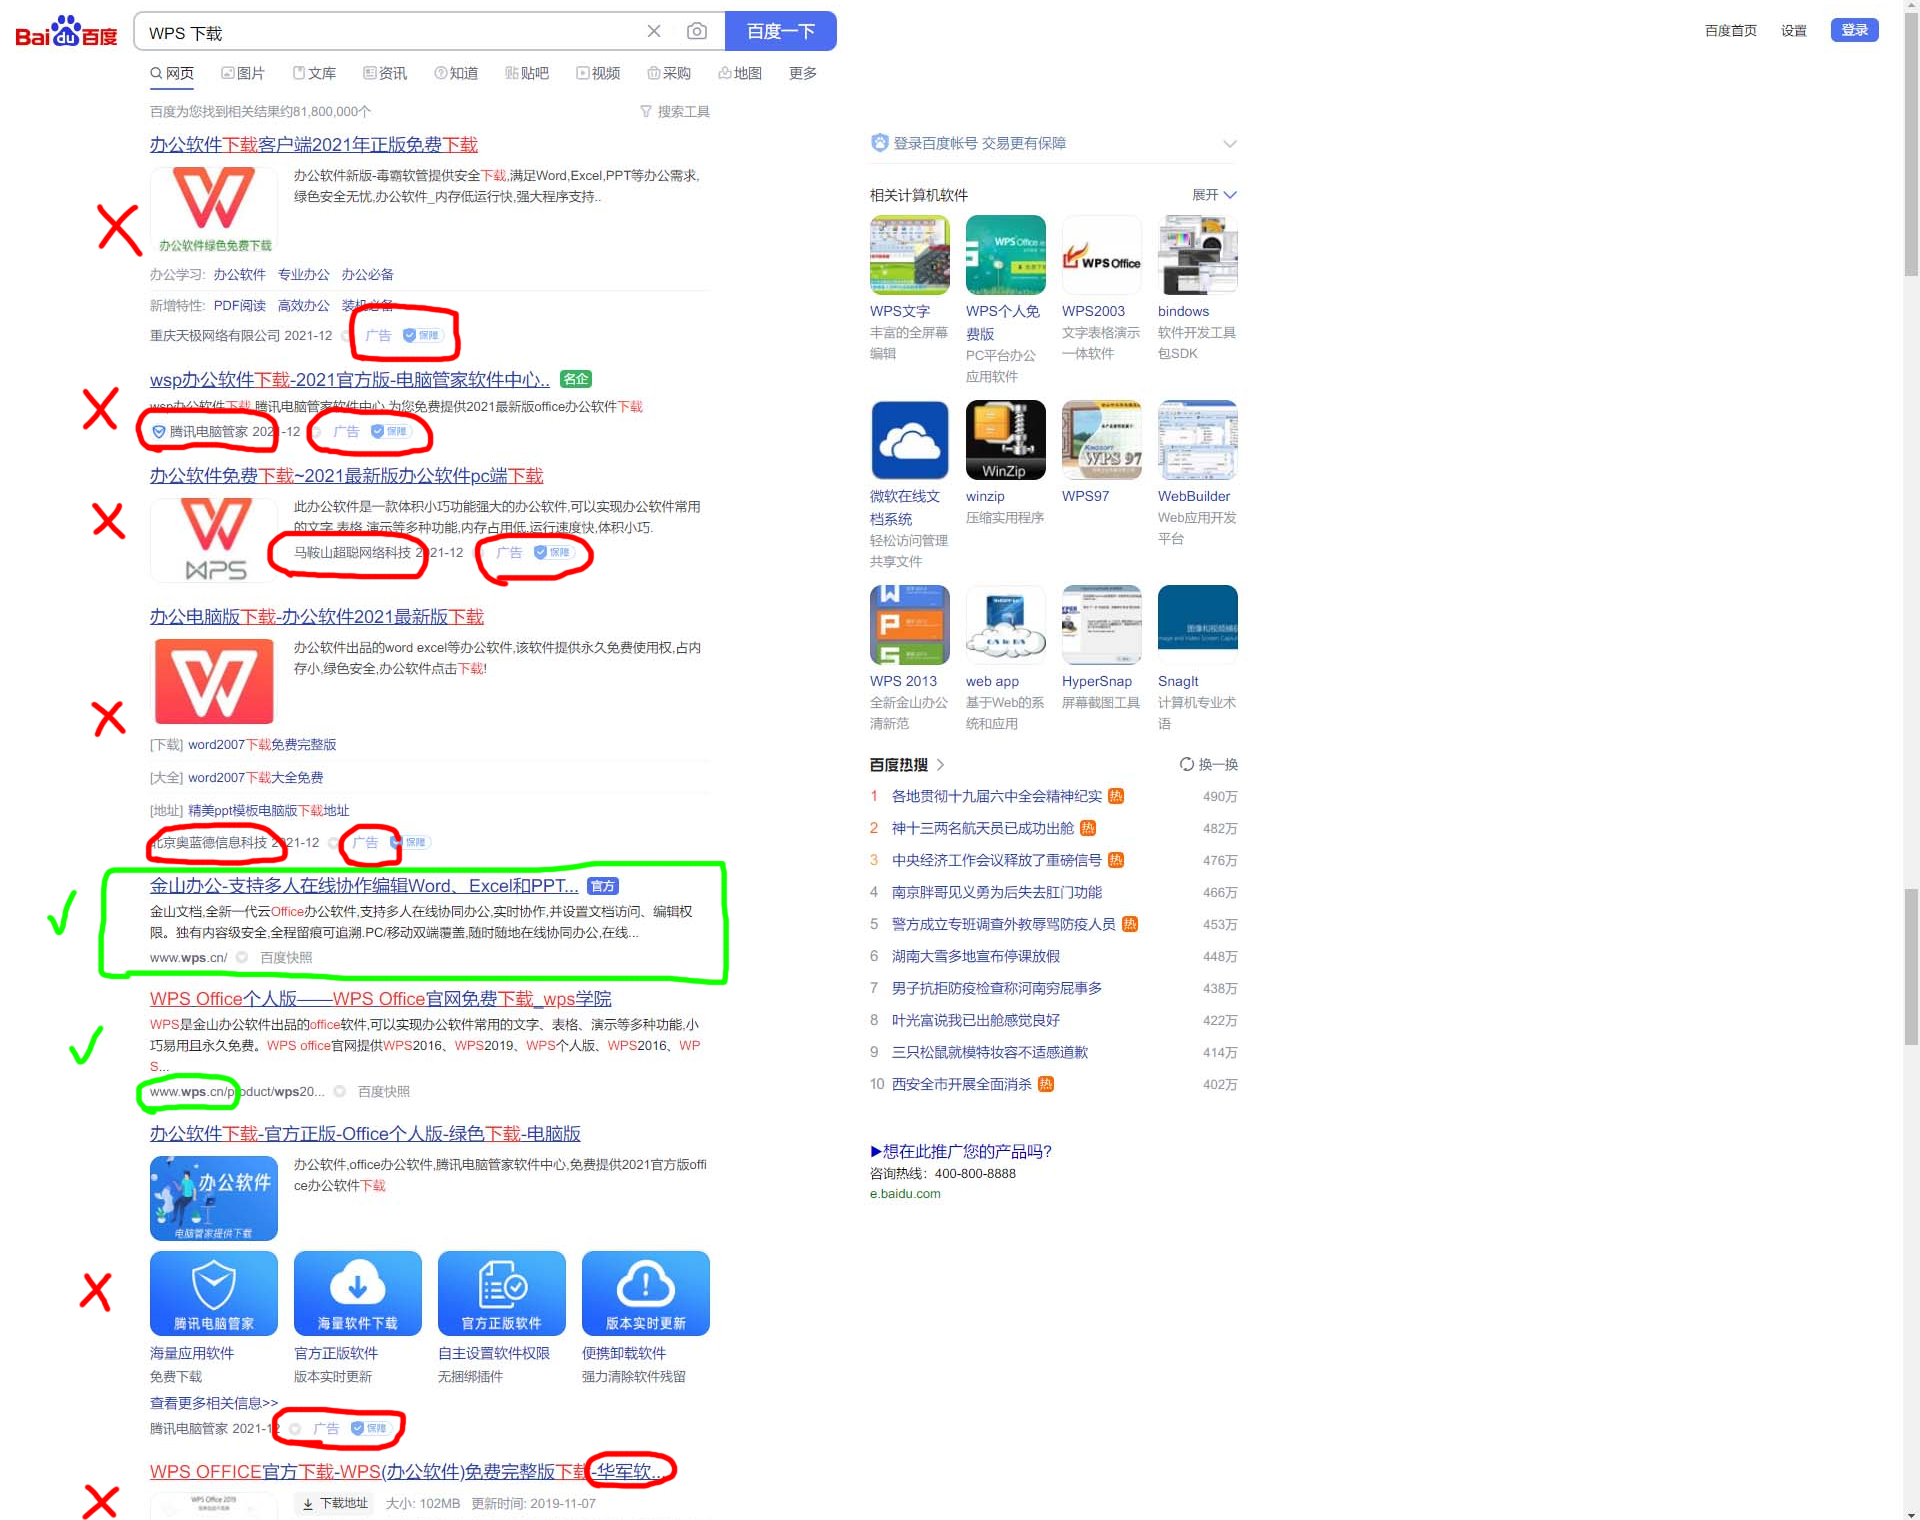
\includegraphics[width=10cm]{assets/Baidu_result.png}
  \caption{百度搜索「WPS 下载」的搜索结果}
  \label{baidu-wps-result}
\end{figure}

在图 \ref{baidu-wps-result} 中,我们搜索「WPS 下载」,然而在结果中:

\begin{itemize}
  \item {\color{Brown1} 第一条是「重庆天极网络有限公司」提供的广告。}
  \item {\color{Brown1} 第二条是「腾讯电脑管家」提供的广告,进去之后八成你会下载到「腾讯电脑管家」而不是「WPS」。}
  \item {\color{Brown1} 第三条是「马鞍山超聪网络科技」提供的广告。}
  \item {\color{Brown1} 第四条是「北京奥蓝德信息科技」提供的广告。}
\end{itemize}

\regcolor{上面这四条全部是广告}。这意味着进入这些页面,你八成下载不到干净的「WPS」,而只能下载到一堆垃圾。

\begin{itemize}
  \item {\color{Chartreuse3} 第五条是 WPS 官网。注意看它的网址是 \texttt{www.wps.cn},这是 WPS 的官方网站。}
  \item {\color{Chartreuse3} 第六条也是官网。}
  \item {\color{Brown1} 第七条又是「腾讯电脑管家」的广告。}
  \item {\color{DarkGoldenrod2} 第八条是第三方下载站「华军软件园」的链接。我们在后面会提到,当官网不可用的时候,怎么从这种第三方下载站下载软件。}
\end{itemize}

鉴别一个网站到底是不是官网,我们主要可以观察这么几个地方:

\begin{itemize}
  \item 看网址。一般官网的网址都是企业或者软件的名字。例如:
  \begin{itemize}
    \item WPS 的官网是 \verb|www.wps.cn|。
    \item QQ 的官网是 \verb|im.qq.com|。微信的则是 \verb|weixin.qq.com|。(腾讯首页:\verb|qq.com|)
    \item 网易云音乐的官网是 \verb|music.163.com|。(网易官网:\verb|163.com|)
    \item ……
  \end{itemize}
  \item 排除法。没有哪个软件厂商的名字是叫做「xx 软件站」「xx 下载站」「xx 软件园」的。带有这些名字的全部是第三方下载站。
  \item 语义判断。一般广告网站的标题都与搜索关键词没有任何实质上的联系。我们不妨再看上面的搜索结果中的前四条广告:
  \begin{itemize}
    \item 第一条:「办公软件下载客户端 2021 年正版免费下载」,只字不提「WPS」或者「金山办公」。(WPS 是金山公司开发的办公软件)
    \item 第二条:「wsp 办公软件下载-2021 官方版-电脑管家软件中心」,挂羊头卖狗肉而且挂错了。
    \item 第三条、第四条类似第一条。
  \end{itemize}
\end{itemize}

进入软件的官方网站之后,我们搜索「全部产品」「软件下载」之类的选项,就可以找到我们所需要的软件的安装包。例如从 WPS 的官网上下载 WPS 软件:

\begin{figure}[htb!]
  \centering
  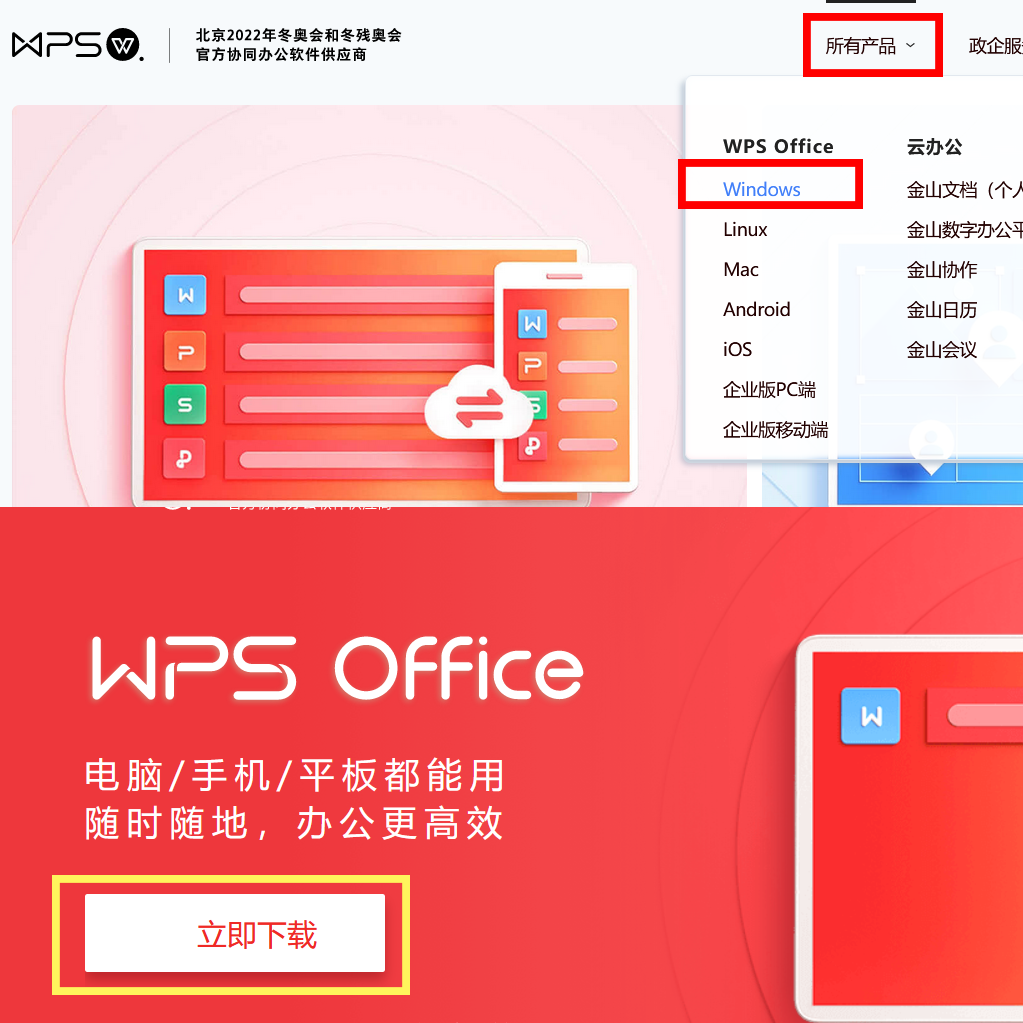
\includegraphics[width=10cm]{assets/Download_WPS.png}
  \caption{从官网下载 WPS}
  \label{download-wps}
\end{figure}

\subsection{直面深渊:第三方软件站}

在某些时候,我们确实找不到一个软件的官网,或者因为这样那样的原因不能去官网下载某个软件。这时,我们将不得不直面深渊,进入「xx 软件园」「xx 软件站」「xx 下载站」这样的网站下载软件。

这种网站一般是可以下载到我们想要的东西的——前提是,你足够小心,不点到那些所谓「高速下载器」「P2P 下载器」的虚假链接。下面我们会手把手实操这个过程。

假设我们要下载「SecureCRT」这款软件。我们在百度上搜索「SecureCRT 下载」,并主动避开那些明显骗人的广告,点击了这个看似还能接受的「华军软件园」网站:

\begin{figure}[H]
  \centering
  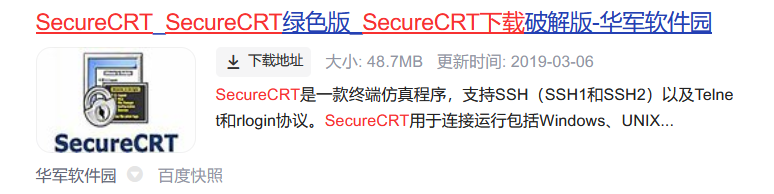
\includegraphics[width=8cm]{assets/Huajun_1.png}
  \caption{「华军软件园」上的「SecureCRT」}
  \label{huajun-1}
\end{figure}

重点来了:\regcolor{进入这个网站,请主动避开所有「高速下载」「极速下载」「P2P 极速下载」这样的按钮,选择「普通下载」「本地下载」这样的按钮}:

\begin{figure}[H]
  \centering
  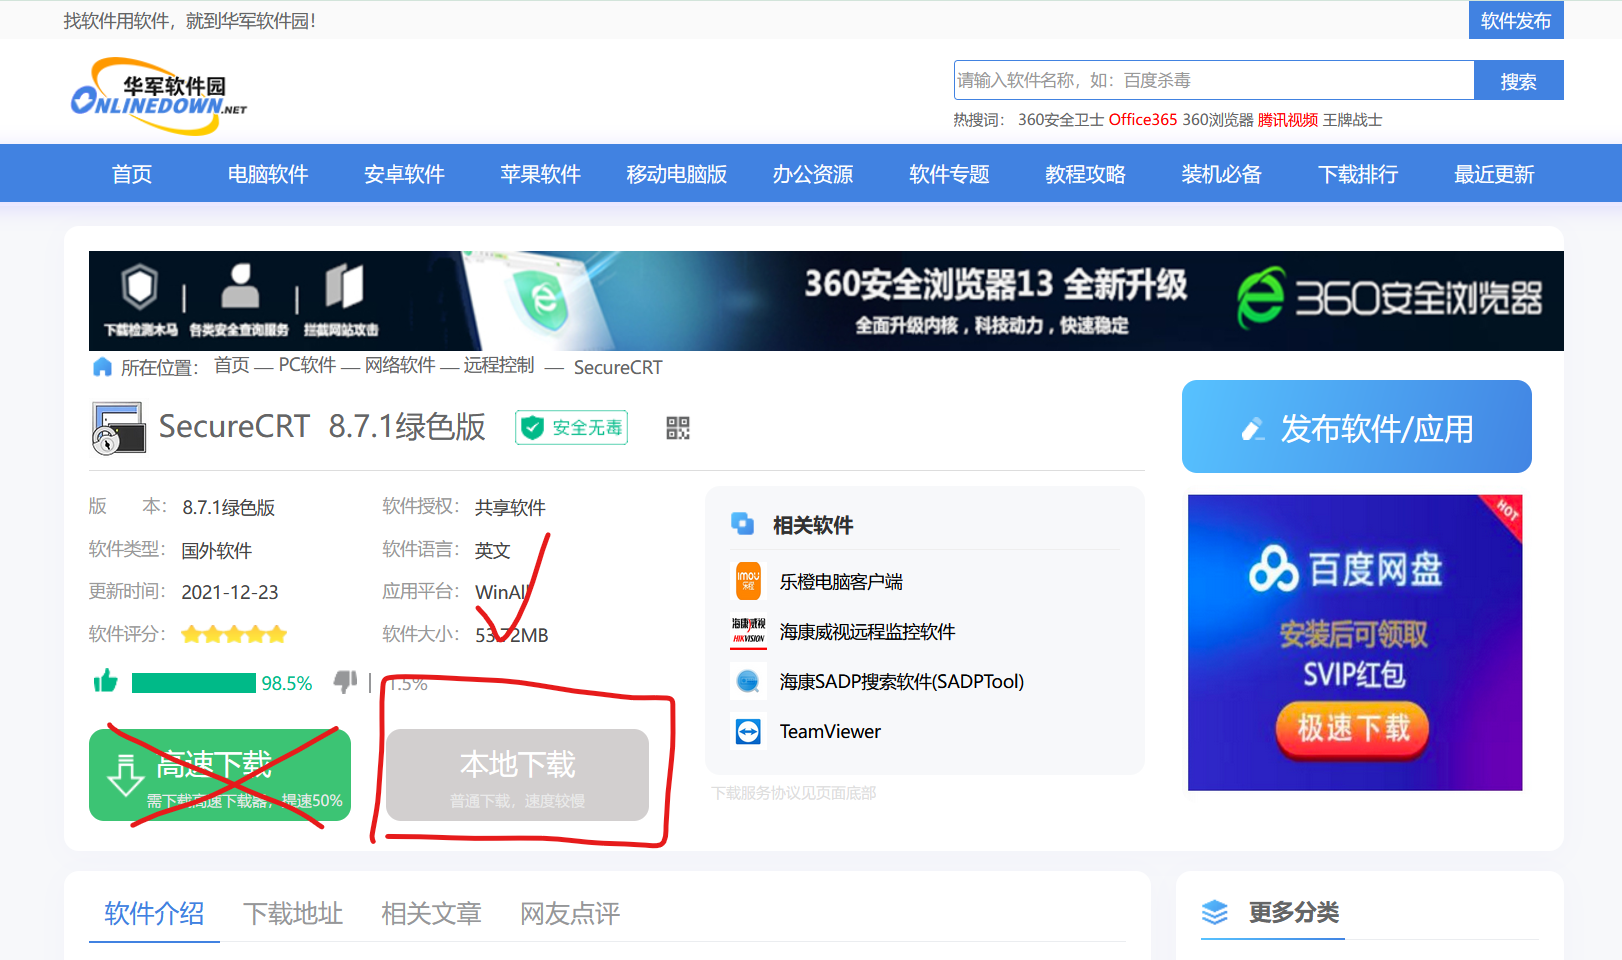
\includegraphics[width=10cm]{assets/Huajun_2.png}
  \caption{不要选择【高速下载】,选择【本地下载】}
  \label{huajun-2}
\end{figure}

点击之后我们会跳转到这样一个「下载地址」的页面。同样地,我们\regcolor{不要点击「需优先下载高速下载器」之下的所有连接,而要点击「普通下载地址」下方的「通用网络下载」或者「电信网络下载」}:

\begin{figure}[H]
  \centering
  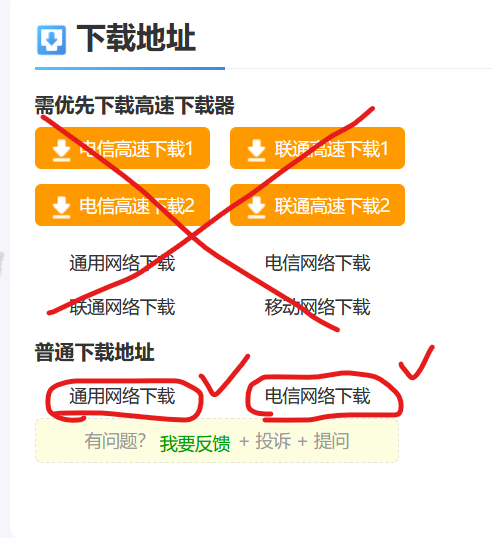
\includegraphics[width=8cm]{assets/Huajun_3.png}
  \caption{不要点击「需优先下载高速下载器」之下的所有链接,选择「普通下载地址」下方的链接}
  \label{huajun-3}
\end{figure}

使用下方两个链接下载到的文件如图 \ref{real-securecrt},体积约 50 MB,符合这个软件的体量;它是一个压缩包,一般解压缩之后就能得到软件的安装包。而使用上方所谓「高速下载」下载到的文件是 \ref{fake-securecrt},体积只有 1 MB,而且是一个不明的「可执行文件」(exe 文件),这是不正常的。在本章的最后,我们会使用一台虚拟机来演示这「高速下载器」会干什么。

\begin{figure}[htb!]
  \centering
  \begin{minipage}{6cm}
    \centering
    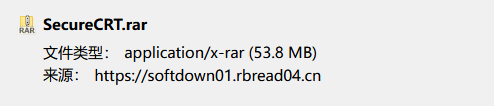
\includegraphics[width=5cm]{assets/Real_SecureCRT.png}
    \caption{点击「普通下载」得到的真正的软件安装包}
    \label{real-securecrt}
  \end{minipage}
  \qquad
  \begin{minipage}{6cm}
    \centering
    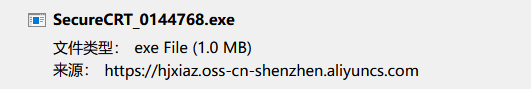
\includegraphics[width=5cm]{assets/Fake_SecureCRT.png}
    \caption{点击「高速下载」得到的假的软件安装包}
    \label{fake-securecrt}
  \end{minipage} 
\end{figure}

\subsection{另辟蹊径:软件公众号及其他小众渠道}

另一种「另辟蹊径」的方法,是通过一些「小众渠道」,例如一些分享软件的微信公众号来下载软件。这不失为一种好方法——那些人们口口相传的优质公众号一般会把常用软件的「干净」安装包分门别类地整理分享,与「xx 下载站」相比,免去了「高速下载器」的烦恼。

但是,这种公众号一般软件不是特别多——你总有一天没法从它们那里找到想要的软件。此外,这些公众号一般使用百度网盘来分享文件,而众所周知百度网盘是对非会员限速的,这必然对使用体验有一定影响。不过总的来说,这依然是一种值得推荐的方法。

\begin{note}
  对于这类公众号,我们并没有做太多的收集,因此无法在此推荐。大家可以在 B 站、贴吧、微博等地方自行寻路。
\end{note}

\subsection{他山之石:第三方的「软件管家」}

除了手动在网上——无论是在官网,从第三方下载站,还是从那些整理网站的公众号上——下载软件的安装包之外,有一些第三方的「软件管家」也能帮助我们找到所需要的软件。这些软件管家有的是电脑厂商所维护的,例如「联想软件管家」「华为软件管家」;有的是一些公司所维护的,比如「360 软件管家」「腾讯软件管家」等(名字不一定是这样,可以类比)。

一般来说,那些由电脑厂商所维护的「软件管家」,往往相对干净、不带「全家桶」式的捆绑;而那些第三方企业维护的「软件管家」,一般都会或多或少地提示用户安装它们的「全家桶」。比如,如果你使用「360 软件管家」,那它一定会用某些手段提示用户去安装「360 安全卫士」以及一系列其他软件。因此,你可以根据自身机器的实际情况,按需选择这样的「软件管家」类 app。

\section{安装软件}

假设经过与流氓网站的「斗智斗勇」,你成功地下载到了某款软件的安装包。取决于软件,你下载到的可能是下面三种文件中的某一种:

\begin{itemize}
  \item 一个光秃秃的 \verb|exe| 文件。
  \item 一个压缩包,例如 \verb|zip| 或 \verb|rar| 文件。
  \item 一个扩展名是 \verb|iso| 的文件。
\end{itemize}

对于第一种情况,我们直接双击这个 \verb|exe| 文件就能启动安装进程。对于第二种情况,我们需要解压缩这个压缩包到某处,然后在解压出来的文件中找到名字类似「\verb|setup.exe|」或「\verb|install.exe|」的程序双击打开。对于第三种情况,我们右击这个 \verb|iso| 文件,选择【打开方式】→【文件资源管理器】,然后在弹出的新窗口中找到名字类似「\verb|setup.exe|」或「\verb|install.exe|」的程序双击打开\footnote{当你这样打开 \texttt{iso} 文件后,这个文件会临时被「映射」成电脑里的一个新「分区」,打开【此电脑】就能发现它。在你安装完成后,可以打开【此电脑】,右键这个分区选择【弹出】来让这个分区消失。}。

启动安装器后,我们一般按提示【下一步】操作即可完成安装。

\begin{note}
  此过程中也要留心!跨过了「高速下载器」的坎,可不要又掉进了捆绑软件的坑。有一些软件在安装程序中也会像「高速下载器」一样勾选了一些捆绑软件、浏览器主页劫持什么的,这些选项可能出现在安装过程中的任何阶段,一定要注意取消勾选再进行下一步。
\end{note}

在安装过程中需要特别注意的一件事,便是「软件安装位置」,即安装包把软件自身的各种文件「释放」的位置。

在上一章中我们提到过,不要把大量的软件安装在 C 盘——安装到 D 盘或其他磁盘分区是更好的选择。一般来说,软件默认会把自己「释放」在以下两个路径之一:

\begin{verbatim}
  C:\Program Files\<厂商名字>\<软件名字>\
  C:\Program Files (x86)\<厂商名字>\<软件名字>\
\end{verbatim}

在上一章中我们提到了「快捷方式」,在你的电脑桌面上就有许多软件可执行文件的快捷方式。右键它们选择【属性】,你就能看到这些已经安装的软件的位置。看看它们中的一些是不是在 \verb|C:\Program Files\| 或者 \verb|C:\Program Files (x86)\| 下?

\verb|Program Files| 和 \verb|Program Files (x86)| 这两个文件夹,即是系统预置的两个用来安装 app 的文件夹,都位于 C 盘根目录下。然而,我们希望把软件安装到 D 盘。这里推荐一个简单好用的方法:直接将默认路径中的 \verb|C:| 改成 \verb|D:|。例如:

\begin{verbatim}
  D:\Program Files (x86)\Tencent\QQ\
\end{verbatim}

这就是在 D 盘安装 QQ 软件的一个很合适的路径。这样做能保持一个比较干净的目录结构。你的 D 盘下会因此多出 \verb|Program Files| 和 \verb|Program Files (x86)| 这样的两个文件夹,用来专门在 D 盘安装软件。

\begin{figure}[htb!]
  \centering
  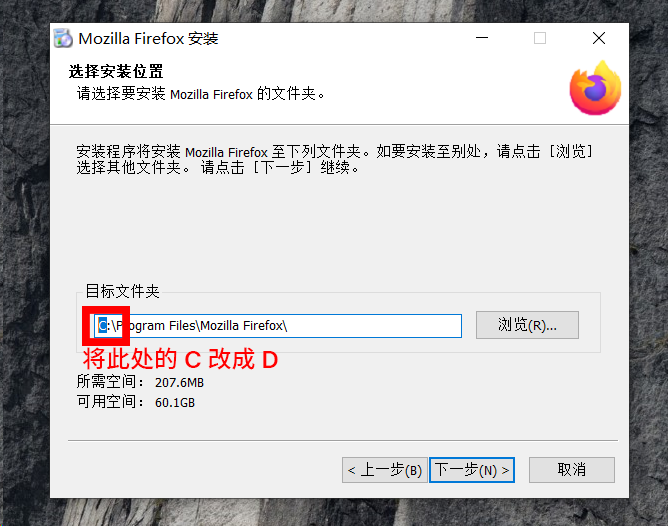
\includegraphics[width=8cm]{assets/Change_C_to_D.png}
  \caption{一般把这个 \texttt{C:} 改成 \texttt{D:} ,就能得到一个不错的 D 盘安装软件的路径}
  \label{change-c-to-d}
\end{figure}

如图 \ref{sogou-install} 所示,有一些软件的安装包不是「下一步」型的,而只有一个「立即安装」的按钮。一般这种情况,可以展开「自定义安装」之类的选项,然后更改软件的安装位置。

\begin{figure}[htb!]
  \centering
  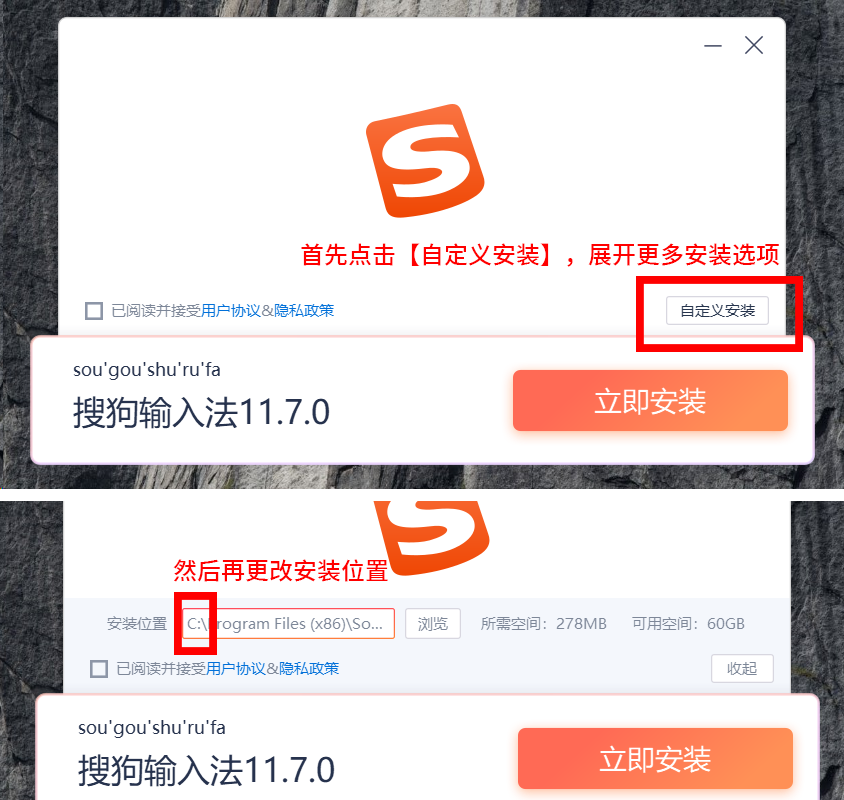
\includegraphics[width=8cm]{assets/Sogou_change_directory.png}
  \caption{对于只有一个「立即安装」按钮的安装包,一般找到「自定义安装」的选项展开后即可更改安装位置}
  \label{sogou-install}
\end{figure}

\section{软件收费、破解和自由软件}

很多软件是需要购买的,包括 Windows 系统本身(一般你购买电脑时,电脑厂商已经帮你出了买 Windows 这部分钱)。常见的专业软件,从平面设计领域的 Adobe 家族的 Photoshop、Premiere Pro,工程领域的 Autodesk 家族的 AutoCAD、3ds MAX,到开发领域的 JetBrains 家族的 IDEA、PyCharm,甚至于我们每天都在用的 Word 和 PowerPoint,这些软件全部都需要付费购买。图 \ref{buy-adobe} 是购买正版 Photoshop(俗称的 PS)软件的页面——定价 888 元一年。

\begin{figure}[htb!]
  \centering
  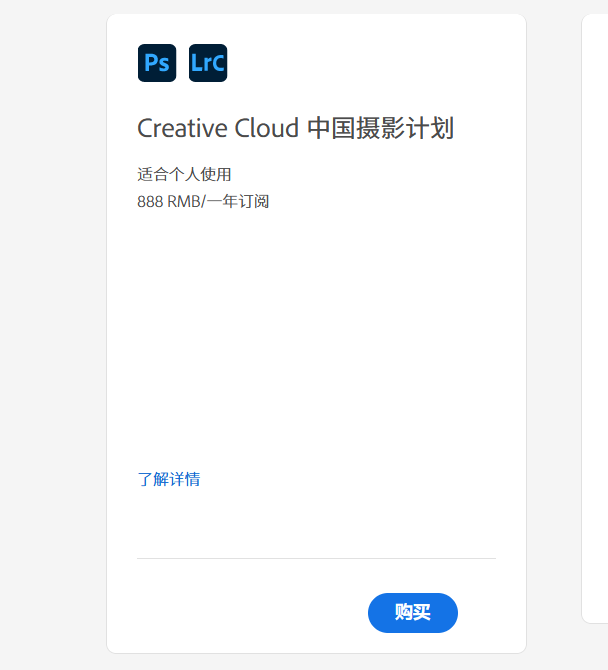
\includegraphics[width=6cm]{assets/Adobe.png}
  \caption{Adobe 的「Creative Cloud 中国摄影计划」套装,包含 Photoshop 和 Lightroom Classic 两款软件,定价 888 元一年。}
  \label{buy-adobe}
\end{figure}

而由于这样或那样的原因,我们在实际生活中,或多或少都在「没有付费而白嫖这些软件」。这是因为我们使用的这些软件被「破解」了。破解之后,软件的计费功能失效,原本收费的软件通过某种方式变成了可以免费永久使用的软件。大体上,网上流传的破解软件一般有这么两种形式:

\begin{itemize}
  \item 一种是已经完全破解了的收费软件。这种软件已经经过修改,安装包往往也是民间自行制作的,可以直接走正常流程安装,安装后打开就可以无限制地使用。例如一些 Adobe 软件破解版套装。
  \item 另一种是使用收费软件的试用版本安装软件,再外加「破解补丁」。这种软件的安装包依然是使用官方原版的安装包,安装完成之后,通过某种「打补丁」的方式来外挂「欺骗」这官方原版的软件,让原版软件以为用户已经购买,从而解锁全部的功能并让用户无限制使用。常见的 Office 软件的破解、Autodesk 软件的破解都属于此类。
\end{itemize}

使用破解软件终究是一件「上不得台面」的事情。一般来说,如果你使用破解软件作为私下的个人使用、学习,软件厂商大多是不会进行追究的。但是,如果你将破解软件(或者说,盗版软件)用于商业用途,那必然迟早会受到追究。尽管实际生活中软件厂商维权的积极程度各有差异,尽管大家会因为各种各样的原因不得不去使用盗版和破解,但我们仍然呼吁大家支持正版软件,万不得已使用盗版、破解软件时,仅作为非商业的个人和学习用途。

与那些用来盈利的商业软件不同,「自由软件」不仅是「免费」(Free as in `free beer')的,而且是「自由」(Free as in `free speech')的。对于自由软件,人们不仅可以无偿使用,还能自由地复制、分发,甚至是在一定条款之下修改它们。自由软件的原始代码是公开的,下载使用是免费的,开发者是多元包容的。近些年来,自由软件作为一种新浪潮在互联网上的发展不断壮大,自由软件在越来越多的领域开始出现。

在今天,一些自由软件已经开始动摇过去一些不可或缺的商业软件的地位。我们鼓励大家在实际使用电脑的过程中,多多尝试、使用一些优质自由软件。在《Missing》的后续章节中,我们会推荐一批各个领域的优质软件,其中就有许多自由软件的身影。

\section{UWP 应用和 Microsoft Store *}

作为 Windows 亲爹的微软早在数年前就意识到,Windows 系统下一直缺少一个官方维护的、像 Apple 的 App Store 那样的「集中化」的软件中心,用户下载软件只能像上文那样上网去苦苦找寻。彼时的微软公司正打算进军手机行业,想要和安卓与 iOS 形成「三足鼎立」之势,微软于是心想:不如弄一种新的 app 格式,这种新的 app 不仅能在我们的 Windows 电脑上运行,还可以在手机上运行;然后我们再顺带弄一个全是这种新格式 app 的应用商店,可谓一举两得。于是微软就这么干了:这种新的 app 格式叫做「通用 Windows 平台应用」(Universal Windows Platform,简称「UWP 应用」),这个应用商店就是我们电脑里的「Microsoft Store」:

\begin{figure}[H]
  \centering
  
\includegraphics[width=5cm]{assets/MS_Store_1.png}
  \caption{Windows 10 中的 Microsoft Store}
  \label{ms-store-in-windows-10}
\end{figure}

可是,时过境迁:微软终究没有能在手机市场打下一片江山,微软做的手机系统最终在近两年宣布「谢幕」。可是微软心想,这「UWP 应用」的先进构想和 Microsoft Store 不能开了头就没了尾,因此它们直到今天依然被保留在 Windows 系统之中。

如果你有打开过「Microsoft Store」,如图 \ref{ms-store},你会发现,其中有一些应用是我们日常生活中的常用应用,而另外的大多数应用,我们都从来没有听说过。而事实上,如果你去仔细查看那里面的常用应用,会发现它们往往更新得没有官网勤快,有些甚至已经停止了更新。

\begin{figure}[htb!]
  \centering
  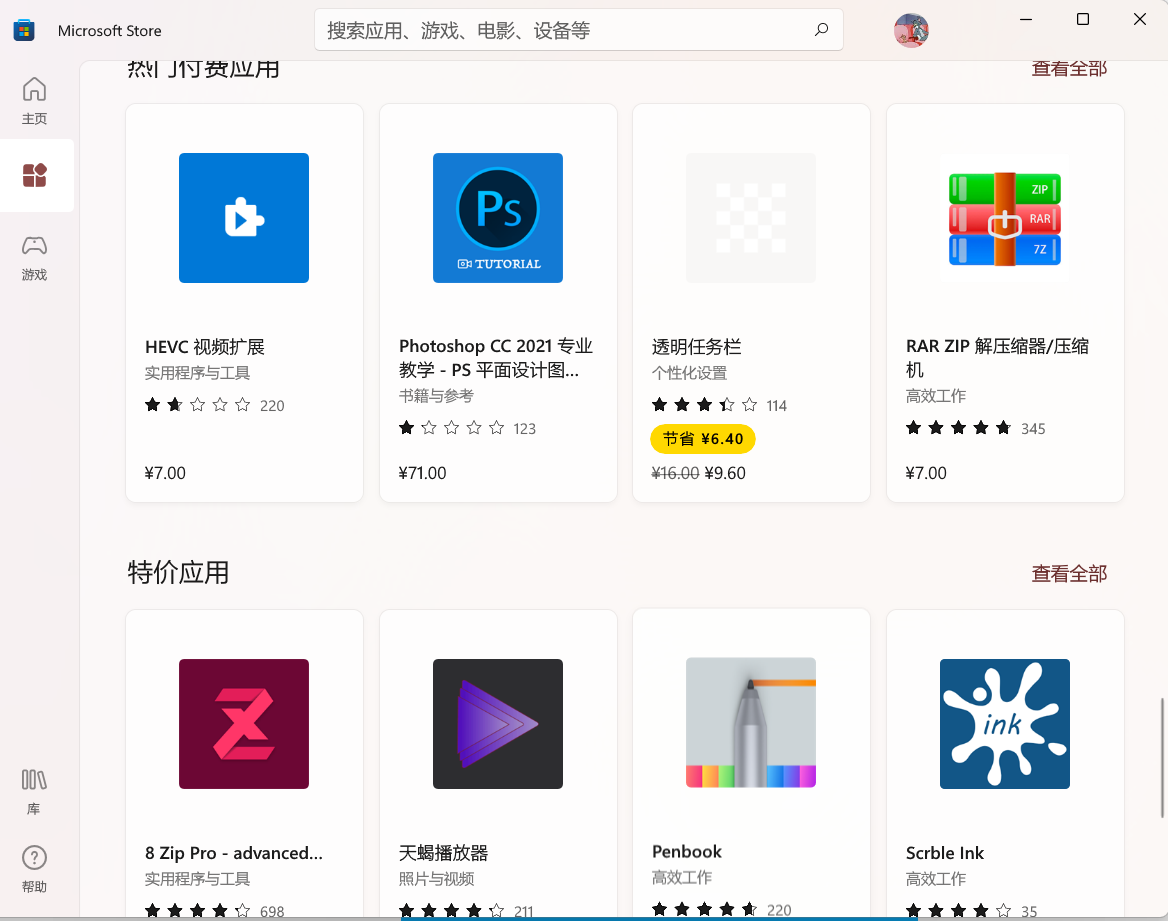
\includegraphics[width=10cm]{assets/MS_Store_2.png}
  \caption{Microsoft Store 的界面}
  \label{ms-store}
\end{figure}

事实上,这就是 Microsoft Store 的现状:作为推广「UWP 应用」的第一线,它没有什么很拿得出手的「杀手锏」;作为一个「xxx 软件中心」的替代品,它的应用相当不全。微软在 Microsoft Store 和 UWP 应用上充满了雄心壮志,却最终落得今天的结局。

\section{演示:「高速下载器」到底会干什么}

\begin{warning}
  \textbf{请不要在自己电脑上尝试打开这种「高速下载器」!}
\end{warning}

在上文中我们演示下载「SecureCRT」时,如果点选了「高速下载」,会得到如图 \ref{gao-su-downloader-1} 的一个只有 1 MB 的可执行文件:

\begin{figure}[H]
  \centering
  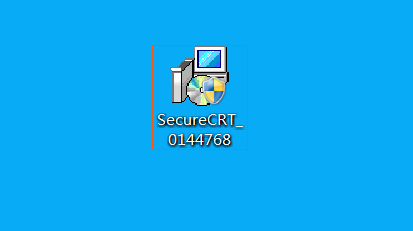
\includegraphics[width=5cm]{assets/Gao_su_1.png}
  \caption{下载到的「高速下载器」,一般来说体积在 1 MB 左右}
  \label{gao-su-downloader-1}
\end{figure}

双击这个「高速下载器」,弹出的窗口如图 \ref{gao-su-downloader-2}。可以看到,右方有四个捆绑软件的复选框被默认勾选:「360 安全浏览器」「QQ 游戏大厅」「U 号租」「百度网盘」,右下方还有一个「六间房直播」。假设我们足够理智,取消勾选了这里的所有的勾,然后点击「快速安装」。等待进度条跑完之后,则会来到图 \ref{gao-su-downloader-3} 的界面。这个界面上又有两个软件捆绑「绝地求生」和「傲视霸主」,以及一个「使用 360 安全导航」的复选框。

\begin{figure}[htb!]
  \centering
  \begin{minipage}{6cm}
    \centering
    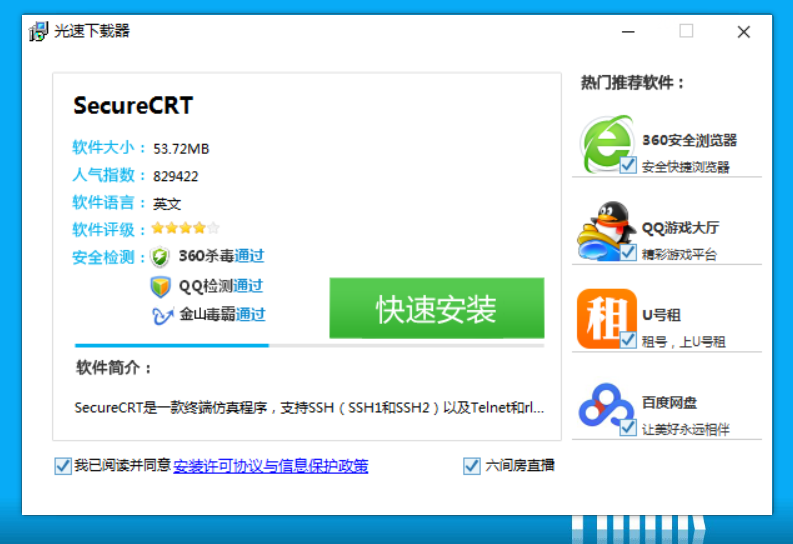
\includegraphics[width=5cm]{assets/Gao_su_2.png}
    \caption{「高速下载器」打开后的界面}
    \label{gao-su-downloader-2}
  \end{minipage}
  \qquad
  \begin{minipage}{6cm}
    \centering
    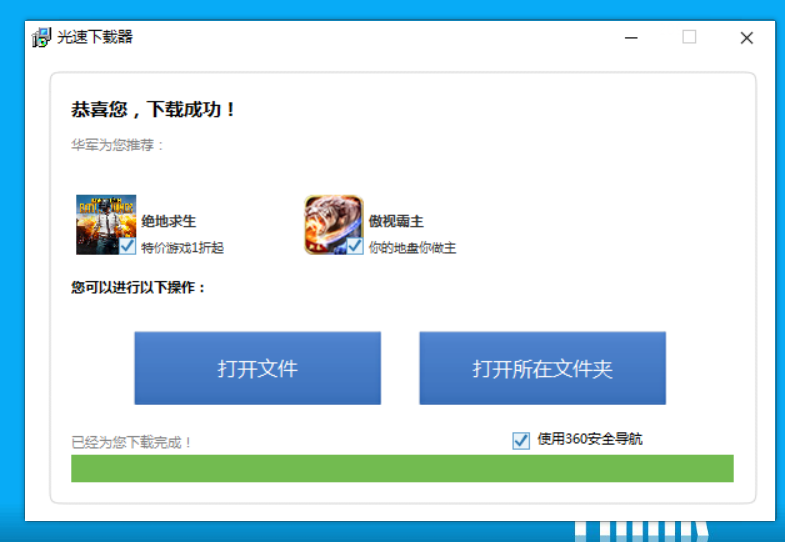
\includegraphics[width=5cm]{assets/Gao_su_3.png}
    \caption{「高速下载器」完成下载后的界面}
    \label{gao-su-downloader-3}
  \end{minipage} 
\end{figure}

全部取消这些复选框,我们点击「打开文件」,终于打开了我们想要的 SecureCRT 的安装包——一个名为 \verb|SecureCRT.rar| 的,体积约 50 MB 的压缩包。而这就是我们直接点选「普通下载」直接就能下载到的东西。

如果我们没有取消上面的这些勾选,那会是什么结局呢?

\begin{warning}
  请勿模仿!
\end{warning}

\begin{figure}[H]
  \centering
  \begin{minipage}{8cm}
    \centering
    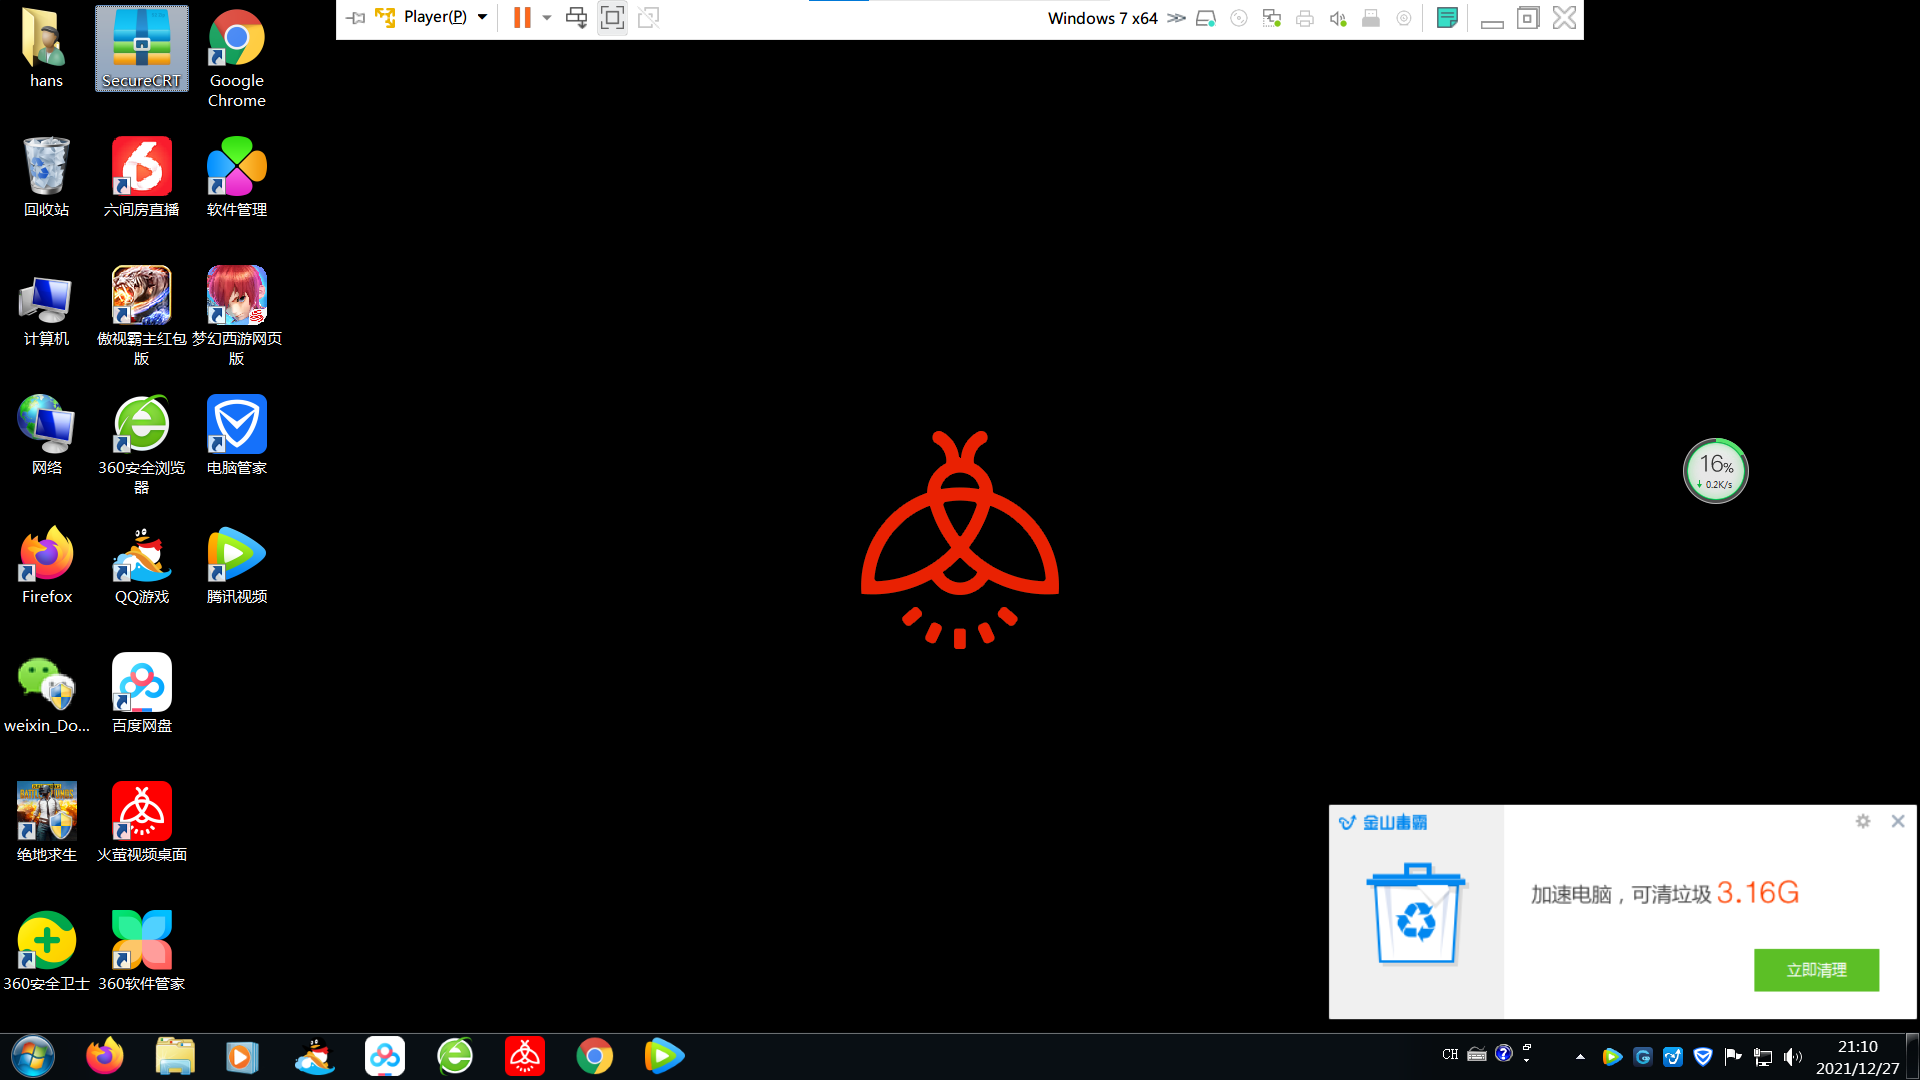
\includegraphics[width=7cm]{assets/Gao_su_4.png}
    \caption{被乱七八糟的软件「占领」的电脑桌面}
    \label{gao-su-downloader-4}
  \end{minipage}
  \qquad
  \begin{minipage}{4cm}
    \centering
    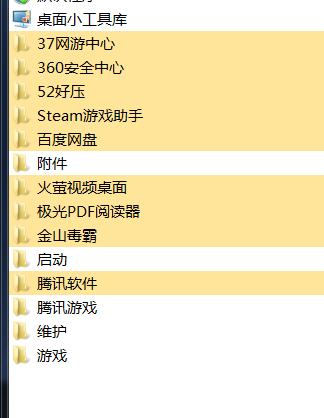
\includegraphics[width=3cm]{assets/Gao_su_5.png}
    \caption{充满各种乱七八糟的软件的「开始」菜单}
    \label{gao-su-downloader-5}
  \end{minipage} 
\end{figure}

我们得到的结论是:

所谓「高速下载器」最后下载到的就是你点击「普通下载」得到的东西,纯属脱裤子放屁。

而「高速下载器」在整个过程中带有许多的捆绑勾选,一旦不留神你的电脑就会被各种垃圾软件充斥。

\begin{note}
  这种流氓的「高速下载器」一般被戏称为「高速下崽器」。
\end{note}

\practice

\begin{enumerate}
  \item 在图 \ref{how-to-download-it-1} 至图 \ref{how-to-download-it-3} 中,怎样操作最不可能下载到垃圾?
  \begin{figure}[htb!]
    \centering
    \begin{minipage}{8cm}
      \centering
      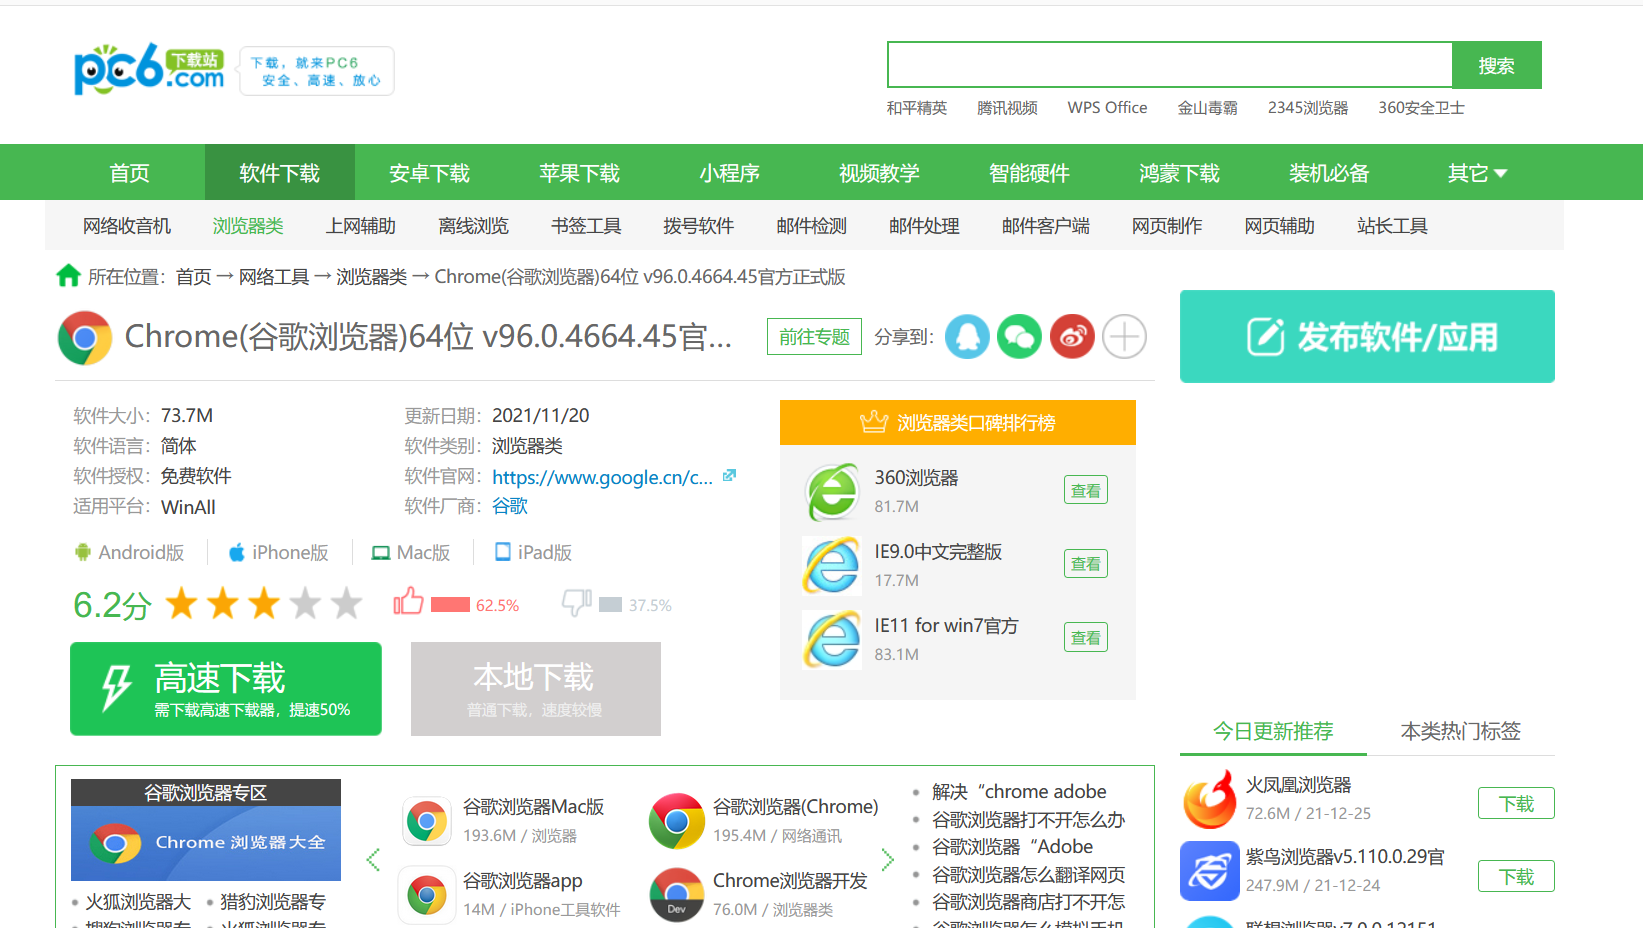
\includegraphics[width=7cm]{assets/How_to_1.png}
      \caption{下载软件「谷歌浏览器」}
      \label{how-to-download-it-1}
    \end{minipage}
    \qquad
    \begin{minipage}{4cm}
      \centering
      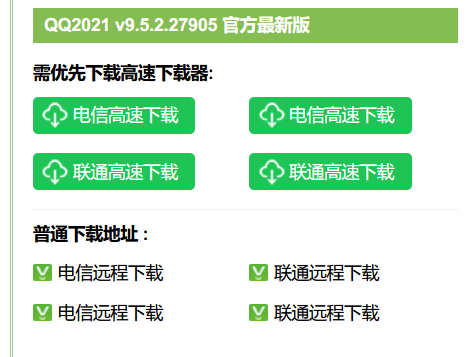
\includegraphics[width=3cm]{assets/How_to_2.png}
      \caption{下载软件「QQ」}
      \label{how-to-download-it-2}
    \end{minipage}    
    \\
    \vspace{1ex}
    \begin{minipage}{12cm}
      \centering
      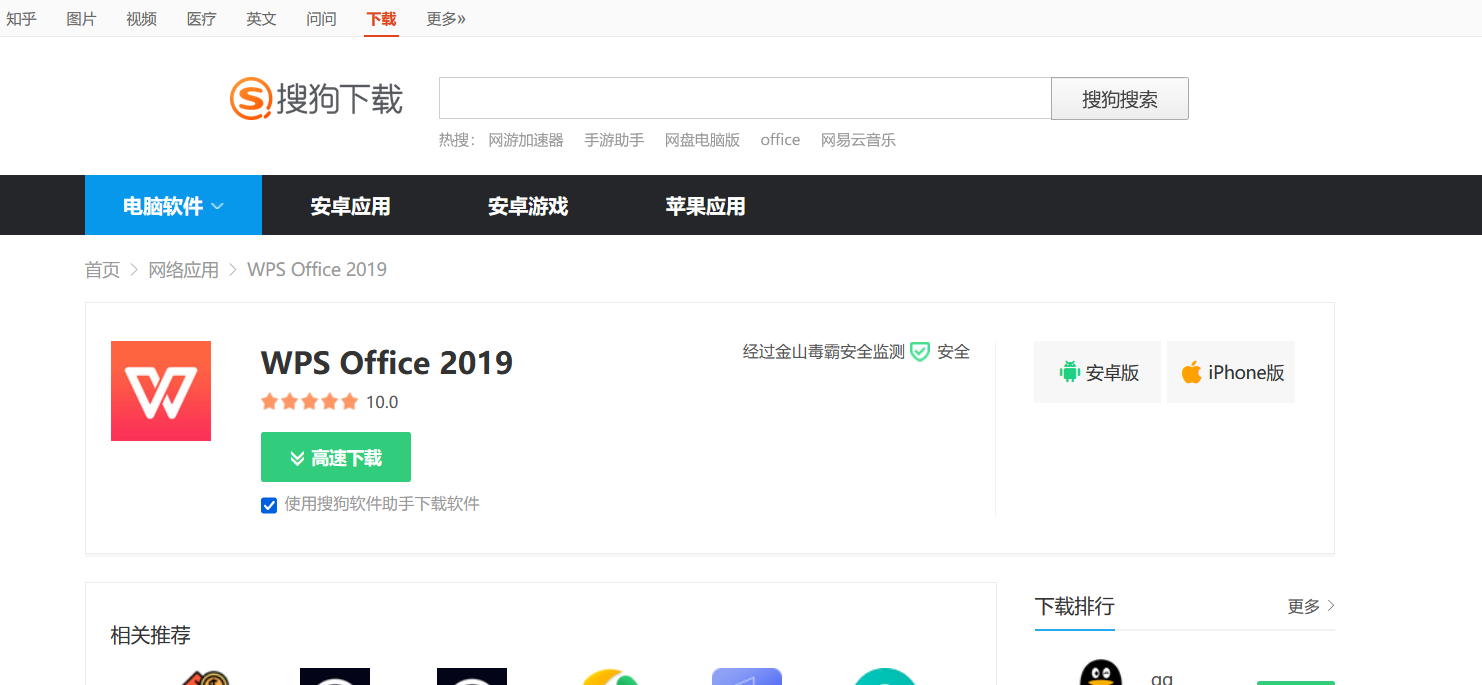
\includegraphics[width=10cm]{assets/How_to_3.png}
      \caption{下载软件「WPS」}
      \label{how-to-download-it-3}
    \end{minipage}
  \end{figure}
  \item 图 \ref{how-to-download-it-4} 的界面中有几个捆绑勾选?
  \begin{figure}[htbp]
    \centering
    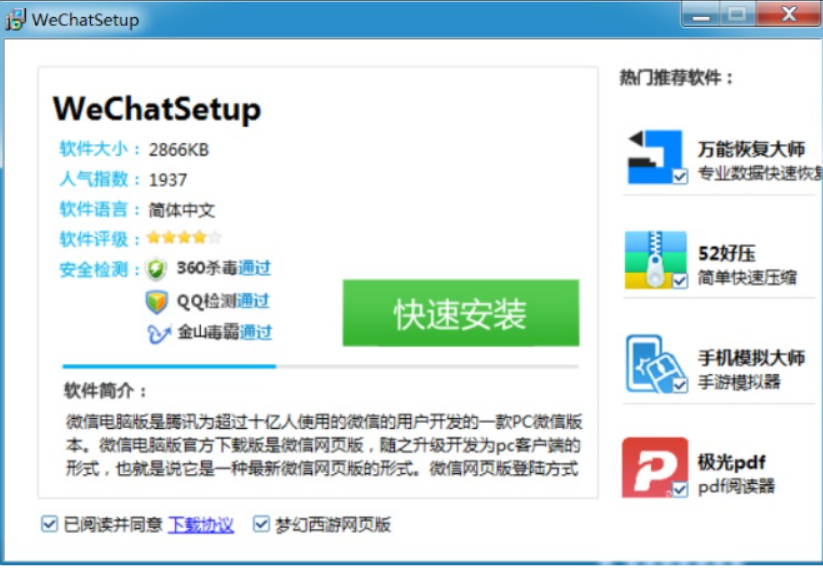
\includegraphics[width=8cm]{assets/How_to_4.png}
    \caption{下载「微信电脑版」时不慎下载到的「高速下载器」}
    \label{how-to-download-it-4}
  \end{figure}
  \item 下载「微信电脑版」,下面三个文件体积中哪一个最可能不是垃圾软件?
  \begin{enumerate}
    \item 640 KB 
    \item 1.1 MB
    \item 150 MB  
  \end{enumerate}
  \item 下面四个软件安装路径,谁最合适?其他的不合适在哪里?
  \begin{enumerate}
    \item 安装 Steam:\verb|C:\Program Files\steam|
    \item 安装微信电脑版:\verb|D:\Program Files (x86)\Tencent\Wechat|
    \item 安装 Vivado:\verb|D:\软件\Xilinx\Vivado|
    \item 安装网易云音乐:\verb|桌面\我的软件\Cloudmusic|
  \end{enumerate}
  \item 假设某个软件已经被安装在了一个地方,我现在想把这个软件放到另一个地方,可以直接剪切移动整个软件的目录到另一个地方吗?
  \item 查看自己电脑上 5 个不同软件的安装位置,并打开它们的安装目录,看一看里面的结构。
\end{enumerate}